% !Rnw root = learnR.Rnw




\marginnote{The screenshots here are for version 0.98.501 of RStudio.}
The url for RStudio is \url{http://www.rstudio.com/}.  Click on the
icon for the downloaded installation file to install it. An RStudio
icon will appear.  Click on the icon to start RStudio.  RStudio should
find any installed version of R, and if necessary start R.  Figure
\ref{fig:rstudio} shows an RStudio display, immediately after starting
up and entering, very unimaginatively, \txtt{1+1}.

\begin{figure*}
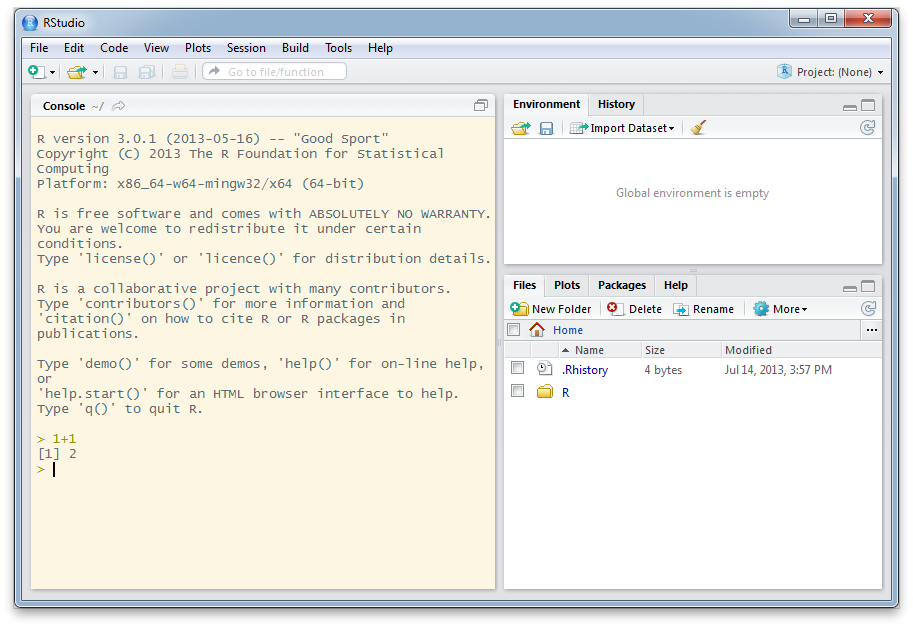
\includegraphics{figs-inc/03i-all4.png}
\caption{Here is shown the RStudio interface, after starting up and
  entering \txtt{1+1}.}\label{fig:rstudio}
\end{figure*}
\pagebreak

Techncally, \marginnote{Extensive and careful RStudio documentation
  can be accessed, assuming an internet connection, from the
  \underline{Help} drop-down menu.  The notes included here are
  designed to draw attention to some of the more important RStudio
  abilities and features.}
RStudio offers an Interactive Development Environment.  It
provides, from a graphical user interface, a range of abilities that
are helpful for organizing and managing work with R.  Helpful features
of RStudio include:
\begin{itemize}
\item The organisation of work into projects.
\item The recording of files that have been accessed from RStudio, of
  help pages accessed, and of plots.  The record of files is
  maintained from one session of a project to the next.
\item By default, a miniature is displayed of any graph that is
  plotted.  A single click expands the miniature to a full graphics
  window.
\item The editing, maintenance and display of code files.
\item Abilities that assist reproducible reporting.
   \marginnote{Alternative available types of markup are R
    Markdown or R HTML or Sweave with LaTeX.}  Markup text
  surrounds R code that is incorporated into a document, with option
  settings used to control the inclusion of code and/or computer
  output in the final document. Output may include tables and graphs.
\item Abilities that help in the creation of packages.
\end{itemize}

\section{The RStudio file menu}

\begin{figure}
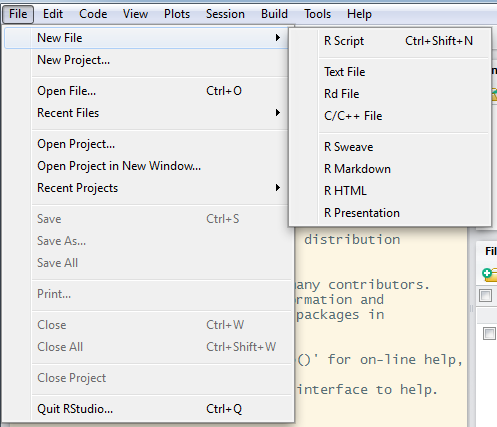
\includegraphics{figs-inc/03i-menu.png}
\caption{The RStudio \underline{File} drop-down menu.  The
  \underline{New File} submenu has been further expanded.}\label{fig:file-menu}
\end{figure}

For now, the RStudio drop-down menus that are of most immediate
importance are \underline{File} and \underline{Help}.  Here (Figure
\ref{fig:file-menu}) is the \underline{File} menu, with the
\underline{New File} submenu also shown.

Here, note the possibility of opening a new R script file, and
entering code into that file. Or, to open an existing R code file,
click on the \underline{Open File...} submenu.

The key combination <CTRL><ENTER> \marginnote{Here, <CTRL> is the
  control key and <ENTER> is the Enter key.}can be used to send code
to the command line.  Code that has been selected will be sent to the
command line.  Or if no code has been selected, the line on which the
cursor is placed will be sent to the command line.

\subsection{Compile a code notebook}

Figure \ref{fig:code-history} shows a script file in the upper left
panel.  The code has been sent to the command line, so that it also
appears in the code history panel on the upper right.

\begin{figure*}
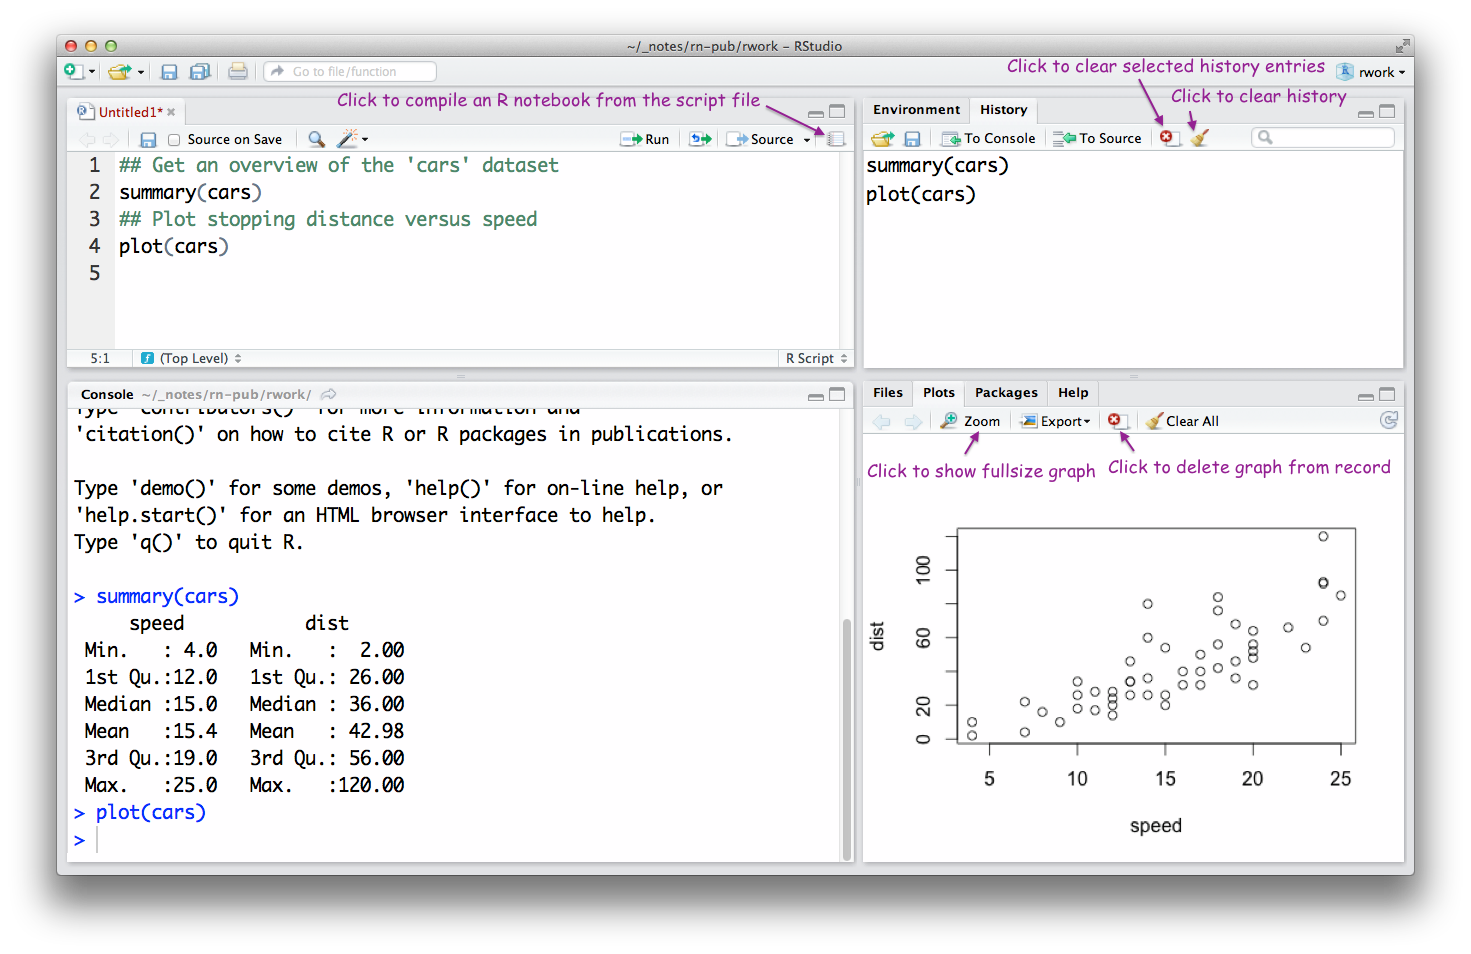
\includegraphics{figs-inc/03i-3panels.png}
\vspace*{-15pt}

\caption{Code from the script window has been sent to the command
  line.}\label{fig:code-history}
\end{figure*}

In Figure \ref{fig:code-history}, take particular note of the icon on
which you can click to create an R notebook. Upon clicking this icon,
the system will ask for a name for the file.  It will then create an
HTML file that has, along with the code and comment, the compluter
output.
\marginnote{For the code that is shown, the HTML file that results
will include the output from \txtt{summary(cars)} and the graph from
  \txtt{plot(cars)}.}  An alternative to clicking on the icon is to
click on the \underline{File} drop-down menu, and then on
\underline{Compile Notebook... }.

\section{Abilities for reproducible reporting}
Markdown editors use simple markup conventions to control how text and
other document features will appear.  For example:
\begin{itemize}
\item[] \txtt{**Help**} or \txtt{\_\_Help\_\_} will be rendered as
\textbf{Help}
\item[] \txtt{*Help*} or \txtt{\_Help\_} will be rendered as {\em Help}.
\end{itemize}

\subsection{R Markdown}
\marginnote{R Markdown, as available under RStudio, is an enhanced
  version of Markdown.  It adds the ability to include R code,
  surrounded by markup that controls what code and/or output will appear
  in the final document.

R users are strongly encouraged to use R Markdown, or another
such markup system that allows embedded R code, for documenting any
work that is more than trivial.  Those who are familiar with
more sophisticated markdown languages may still, for some types
of work, find benefit in the simplicity and speed of working with R
markdown.}

Click on \underline{File} | \underline{New File} | \underline{R
  Markdown...}.  Clicking on HTML (alternatives are PDF, Word), on
\underline{Document} (alternatives are Presentation, Shiny, From
Template) and then on \underline{OK} displays a simple skeleton R
Markdown document thus:
\begin{verbatim}
---
title: "Untitled"
output: html_document
---

This is an R Markdown document. Markdown is a simple
formatting syntax for authoring HTML, PDF, and MS
Word documents. For more details on using R Markdown
see <http://rmarkdown.rstudio.com>.

When you click the **Knit** button a document will
be generated that includes both content as well as
the output of any embedded R code chunks within the
document. You can embed an R code chunk like this:

```{r}
summary(cars)
```

You can also embed plots, for example:

```{r, echo=FALSE}
plot(cars)
```

Note that the `echo = FALSE` parameter was added
to the code chunk to prevent printing of the R
code that generated the plot.
\end{verbatim}
\marginnote[-36pt]{For tutorial purposes, the file can
be processed as it stands.  Click the \underline{Knit HTML}
button to start the process of generating the HTML file.  When
prompted, enter a name for the file.  An HTML file will be
generated and displayed in a browser.}

In actual use, one would edit out the text and R code and replace
it with one's own text and R code chunks, then clicking on
\underline{Knit HTML}. When prompted, enter a name for the file.


\subsection*{R Markdown code chunk options}
The markup that surrounds R code can include instructions on what to
do with R code and/or any output, including tables and graphs. Should
code be executed, should it be echoed, and what output text and/or
tables and/or graphs should appear in the final document?

Here is an example of code with surrounding markup, with the
code chunk options \txtt{fig.width} and \txtt{fig.height}
giving the width and height of the initial figure, and
\txtt{out.width} giving the width to which it should be scaled
in the final document:
\begin{minipage}[t]{1.05\textwidth}
\begin{verbatim}
```{r plotgph, fig.width=7, fig.height=6, out.width="80%"}
plot(cars)
```
\end{verbatim}
\end{minipage}

Giving the code chunk a name, here \txtt{plotgph}, is optional.
\marginnote{Other possible settings include:
  \margtt{echo=FALSE} (do not show code), \&
\margtt{eval=FALSE} (do not evaluate).}
 The \txtt{fig.width} and \txtt{fig.height} settings
  control the size of the output plot, before it is scaled to fit
  within the available line width.  The \txtt{out.width} setting
  controls the width (here given as a percentage of the line
  width) in the final HTML document.  The width may alternatively
  be given in pixels, e.g., `out.width="600px"`.
  
An image from a file {\bf pic.png} that has been generated
separately from the markup R code can be input thus:

\begin{minipage}[t]{1.05\textwidth}
\begin{verbatim}
```{r, out.width="80%"}
knitr::include\_graphics("pic.png")
```
\end{verbatim}
\end{minipage}
  
\subsection*{$^*$Inclusion of HTML in R Markdown documents}
Note also that HTML markup can be included in R Markdown documents.
The following is a less preferred alternative to the
R code \txtt{knitr::include\_graphics("pic.png")} whose use was
demonstrated above:
\begin{verbatim}
<IMG SRC="pic.png" alt="Show this, if no image" STYLE="width: 1200px"/>
\end{verbatim}

The image position can if necessary be adjusted thus:
\begin{verbatim}
<IMG SRC="pic.png" alt="Show this, if no image" STYLE="position:absolute;
TOP:-25px; LEFT:40px; WIDTH:800px; HEIGHT:500px"/>
\end{verbatim}

\subsection*{R Presentation}

Note the R Presentation variant of R Markdown.
To display a simple skeleton  document, click on:
\begin{quote}
\underline{File} | \underline{New File} | \underline{R Presentation}
\end{quote}
An R Presentation document is a specific type of R Markdown document
that is formatted to provide slides that can be displayed using a
browser.

Click on \underline{Knit HTML} to process the document, either as it
stands or after replacing the sample text and code with one's own text
and code.

\subsection{$^*$Other markup types -- HTML,  LaTeX, \ldots}

\subsection*{R HTML}
\marginnote{Also available is reStructuredText (reST), which is an
  extended variant of R Markdown.}

Click on \underline{File} | \underline{New File} | \underline{R HTML}
to display a skeleton HTML document that has embedded R code.
The following shows the markup format:
\begin{verbatim}
<!--begin.rcode fig.width=7, fig.height=6, out.width="600px"
plot(cars)
end.rcode-->
\end{verbatim}

Again, the document that appears can be processed as it stands --
click on \underline{Knit HTML}.

\subsection*{R Sweave: }

Click on \underline{File} | \underline{New
  File} | \underline{R Sweave} to display a template for a LaTeX file.
The web page \url{http://maths-people.anu.edu.au/~johnm/r-book/knitr/} has
files that demonstrate the use of {\em knitr} Sweave type markup.

\subsection{RStudio documentation -- markup and other}

Extensive RStudio documentation is available online.  Click on
\underline{Help} | \underline{RStudio Docs} to go to the relevant web
page. For \underline{R Markdown} and \underline{R Presentation}, note
the documentation files for {\bf Using R Markdown}.  \LaTeX\ users
should note the {\bf Sweave and knitr} documentation files.

\subsection{A strategy for RStudio project management}

RStudio is designed to encourage good project management practices,
using a strategy akin to the following:
\begin{itemize}
\item[] Set up each new project in its own working directory.
\item[] For each project, maintain one or more script files that
holds the code.  Script files can be compiled into "notebooks"
for purposes of keeping a paper record.
\item[] Script files are readily expanded into R Markdown documents
-- a simple form of "reproducible reporting" document.  They can
as required be expanded into a draft for a paper.
\end{itemize}
